%%%%%%%%%%%%%%%%%%%%%%%%%%%%%%%%%%%%%%%%%
% Professional Mathematical Presentation Template
% 
% This template uses the beamer class with the Madrid theme
% and a custom color scheme for a clean, professional look
% that works well with mathematical content.
%%%%%%%%%%%%%%%%%%%%%%%%%%%%%%%%%%%%%%%%%

\documentclass[aspectratio=169]{beamer} % 16:9 aspect ratio (modern)

% Theme settings
\usetheme{Madrid}
\usecolortheme{default}


\definecolor{primcolor}{RGB}{25,50,100} % Dark blue
\setbeamercolor{structure}{fg=primcolor}
\setbeamercolor{frametitle}{bg=primcolor!15, fg=primcolor}
\setbeamercolor{title}{fg=white} % White title text for contrast
\setbeamercolor{subtitle}{fg=white} % White subtitle text
\setbeamercolor{author}{fg=primcolor} % White author text
\setbeamercolor{date}{fg=primcolor} % White date text
\setbeamercolor{institute}{fg=primcolor} % White institute text

% Font settings
\usefonttheme{professionalfonts}
\usefonttheme{serif}

% Package imports
\usepackage{amsmath, amsfonts, amssymb, amsthm} % Math packages
\usepackage{mathtools} % Enhanced math tools
\usepackage{bm} % Bold math symbols
\usepackage{graphicx} % For images
\usepackage{booktabs} % Professional tables
\usepackage{tikz} % For diagrams
\usetikzlibrary{arrows, positioning, matrix, decorations.pathreplacing}

% Use beamer's theorem styles
\setbeamertemplate{theorem}[ams style]
\setbeamertemplate{theorems}[numbered]


% Remove navigation symbols
\setbeamertemplate{navigation symbols}{}

% Custom footer
\setbeamertemplate{footline}{
  \leavevmode%
  \hbox{%
  \begin{beamercolorbox}[wd=.333333\paperwidth,ht=2.25ex,dp=1ex,center]{author in head/foot}%
    \usebeamerfont{author in head/foot}\insertshortauthor
  \end{beamercolorbox}%
  \begin{beamercolorbox}[wd=.333333\paperwidth,ht=2.25ex,dp=1ex,center]{title in head/foot}%
    \usebeamerfont{title in head/foot}\insertshorttitle
  \end{beamercolorbox}%
  \begin{beamercolorbox}[wd=.333333\paperwidth,ht=2.25ex,dp=1ex,right]{date in head/foot}%
    \usebeamerfont{date in head/foot}\insertshortdate{}\hspace*{2em}
    \insertframenumber{} / \inserttotalframenumber\hspace*{2ex} 
  \end{beamercolorbox}}%
  \vskip0pt%
}

% Title information
\title[DRL]{Deep Reinforcement Learning can promote sustainable human behaviour in common-pool resource problem}
\subtitle{Koster et al. 2025}
\author[Longye]{Longye Tian \\ \texttt{longye.tian@anu.edu.au}}
\institute[ANU]{Australian National University\\ School of Economics}
\date{March 27th, 2025}
\DeclareFontFamily{U}{mathx}{\hyphenchar\font45}
\DeclareFontShape{U}{mathx}{m}{n}{
      <5> <6> <7> <8> <9> <10>
      <10.95> <12> <14.4> <17.28> <20.74> <24.88>
      mathx10
      }{}
\DeclareSymbolFont{mathx}{U}{mathx}{m}{n}
\DeclareMathSymbol{\bigtimes}{1}{mathx}{"91}

\begin{document}

% Title frame
\begin{frame}
  \titlepage
\end{frame}

% Outline frame
\begin{frame}{Outline}
  \tableofcontents
\end{frame}
\section{Motivation}
\begin{frame}{Motivation - A canonical trust problem}
The canonical trust problem is
\begin{itemize}
\item resources are distributed from a common pool to a group of people
\item People choose to replenish the pool or not
\item Current solutions to this problem is people can self-organize via contracts, sanctioning etc. 
\item Unanswered for question about how resources can be allocated by a principal agent or social planner in ways that incentive trust, when self-organization is not permitted.
\end{itemize}
\textbf{Research Question: Whether there exist top-down resource allocation mechanism that can lead to a sustainable, inclusive economy, for example by encouraging recipients to reciprocate because they consider allocation to be beneficial, fair and transparent.}
\end{frame}

\begin{frame}{Common Pool Resource Problem}
\begin{figure}
    \centering
    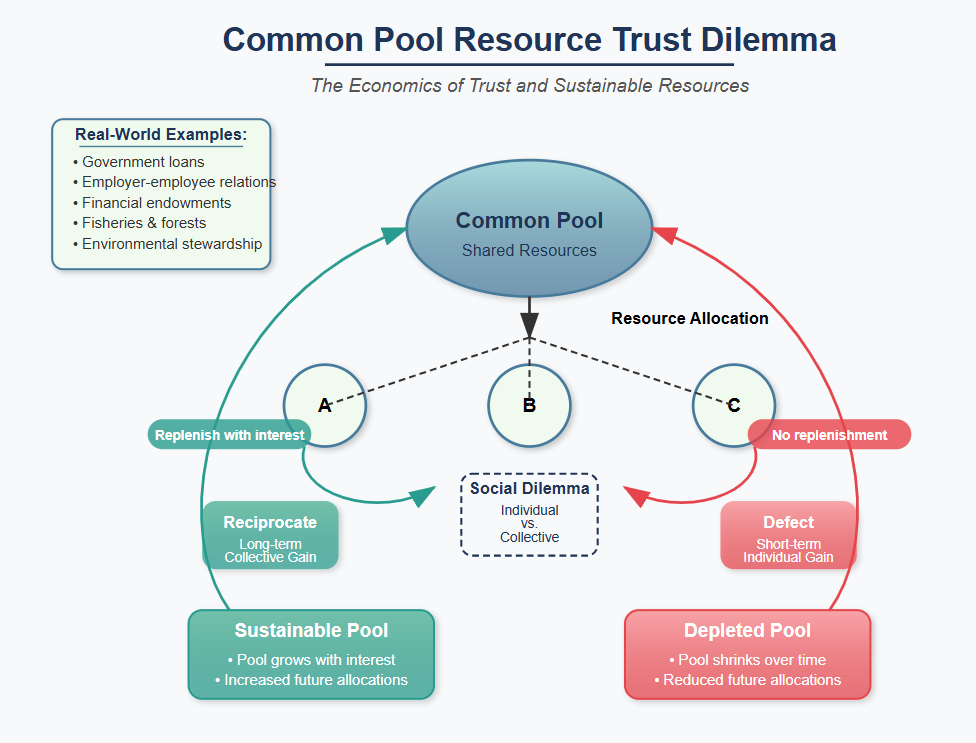
\includegraphics[width=0.6\linewidth]{Literature Reading/RL/CPR problem.png}
\end{figure}
    
\end{frame}

\begin{frame}{Structure of the paper}
    
\end{frame}


\begin{frame}{Main Result}
\begin{enumerate}
    \item Collect data from human players under various allocation mechanism
    \item \textcolor{blue}{Train the neural network, behavioral clones to imitate human behaviors}
    \item Behavioral clones create more data for the RL agents to design a mechanism 
    \item Adopt that RL-based mechanism to real human to validate its performace
    \item Interpret the RL-based mechanism.
\end{enumerate}
\end{frame}

\begin{frame}{Key points}
\begin{itemize}
    \item Behavioral Clone is something I really like
    \item This is an more applied paper 
\end{itemize}
    
\end{frame}



\begin{frame}{Discussion}
\begin{itemize}
    \item the use of behaviour clone compared to economic agent (performance in static environment vs. structural change, policy shift)
    \item What happens at equilibrium (What if we have RL agent designing mechanisms and RL players participate the game?)
\end{itemize}
    
\end{frame}


\begin{frame}{Not so good part}
\begin{itemize}
    \item Not very robust 
\end{itemize}
    
\end{frame}
\end{document}
